\subsection{Esquema de dependências}
O Physimulation depende de três bibliotecas: Chipmunk, Gosu e Glade. O programa começa com a leitura de dados com a interface criada com o Glade. Após a leitura, 
os dados lidos são convertidos em informações para que o Chipmunk possa processar e devolver o resultado da simulação. Os resultados das simulações são animadas 
com o Gosu. Toda interação entre as bibliotecas é feito com a linguagem Ruby. \\

A figura 1 representa um resumo do esquema de dependências entre as bibliotecas e o fluxo da dados da simulação.

\begin{figure}[!htbp]
  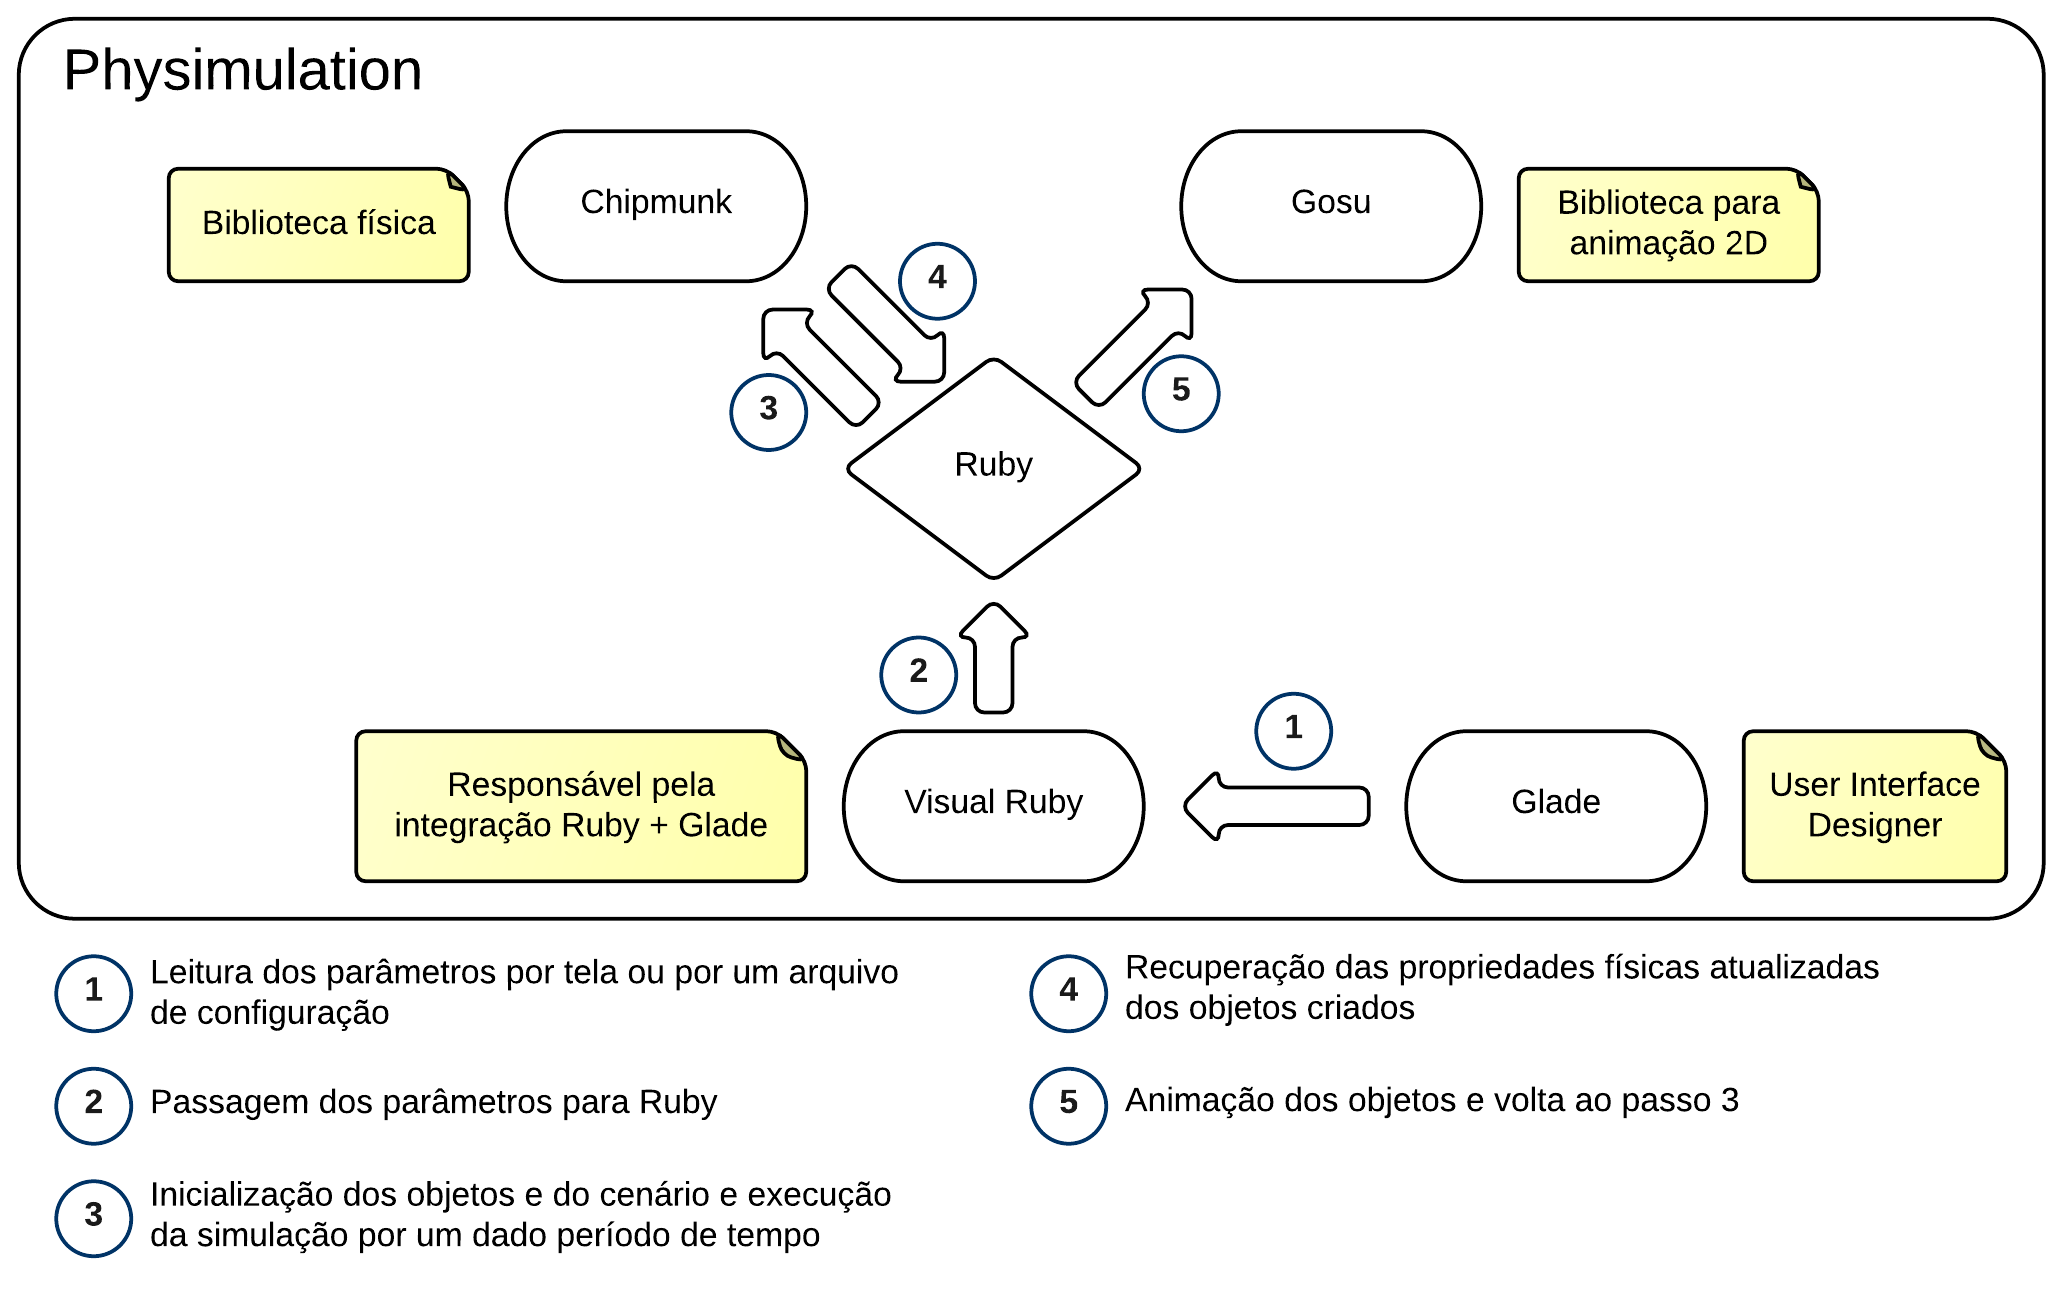
\includegraphics[scale=0.2]{EsquemaDependencia.png}
  \caption{Esquema de dependências do Physimulation}
\end{figure}

Nas seções seguintes mostraremos algumas características das ferramentas utilizadas no Physimulation.

\subsection{Ruby}
É a linguagem de programação utilizada no Physimulation para integrar todas as bibliotecas.
Ruby é puramente orientado a objetos, ou seja, tudo é objeto em ruby. O Código 1 apresenta um exemplo de um método dos números, criado no Physimulation, onde o 
número é convertido de radianos para grau:

\begin{lstlisting}[language=Ruby, caption=Conversão de radianos em graus]
  def graus = 3.14.radians_to_degrees
\end{lstlisting} 

\ \\
Ruby também permite ao programador alterar partes da própria linguagem, tornado-a flexível. Podemos alterar comportamentos de classes ou objetos 
em tempo de execução. Um exemplo é listado no Código 2, onde adicionamos o método radians\_to\_degrees na classe Numeric: 

\begin{lstlisting}[language=Ruby, caption=physics.rb ]
class Numeric
 def radians_to_degrees
    self * 180 / Math::PI
    end
 end
\end{lstlisting} 

\ \\
Outro recurso interessante utilizado no Physimulation são blocos. Os Blocos podem ser anexados a qualquer método descrevendo como deve ser 
o comportamento da execução deste método. O Código 3 mostra um exemplo do uso de blocos em Ruby. Neste exemplo, passamos um bloco ao método velocity\_func 
par atualizar a velocidade do objeto em relação a força gravitacional da lua e da terra:

\begin{lstlisting}[language=Ruby, caption=RocketSimulation.rb]
    self.body.velocity_func { 
      |body, gravity, damping, dt|

      @earth_a = get_earth_acceleration(self)
      @moont_a = get_moon_acceleration(self)

      def self_a = vec2(@earth_a + @moon_a, 0)

      self.body.update_velocity(self_a, damping, dt)
    }
\end{lstlisting}

\subsection{Simulação com Chipmunk}
Chipmunk é uma biblioteca física 2D escrita em C que permite criar objetos convexos e segmentos que se interagem em um ambiente físico. Para criar os 
objetos para simulação é preciso definir as propriedades físicas e a forma do objeto. Após a criação precisamos adicioná-la à um ambiente físico para podermos 
iniciar a simulação.

Para criar o objeto é necessário primeiro definir o corpo. O corpo do objeto pode ser estático ou não. Um corpo estático é o corpo que não precisa de
massa e momento de inércia pois não é influenciado por nenhuma força física, se mantendo fixo no ambiente. Código 4 mostra como criar o corpo de um objeto:

\begin{lstlisting}[language=Ruby, caption=physics.rb]
  if options[:static]
    @body = CP::StaticBody.new
  else
    @body = CP::Body.new(massa, momento_inercia)
    @body.v = velocidade
    @body.w = velocidade_angular
  end

  @body.p = vetor_posicao
  @body.a = angulo
\end{lstlisting} 

\ \\
Após a definição das propriedades físicas de um objeto, é necessário definir a forma do objeto para o Chipmunk tratar as colisões. No Chipmunk é 
possível criar três formas primitivas: Segmentos, círculos e polígonos convexos. No Physimulation criamos as formas de acordo com os parâmetros enviados
pela tela inicial. É necessário passar o corpo associado a forma no momento da criação. O código 5 mostra como são criados as formas no Physimulation:

\begin{lstlisting}[language=Ruby, caption=physics.rb]
  def self.factory(body, params = {})
    # Se existe um raio, criamos um circulo
    if params.has_key? :radius
      return Shape::Circle.new(body, 
        params[:radius], 
        Vec2::ZERO)
    # Se existe uma espessura, criamos um segmento
    if params.has_key? :thickness
      return Shape::Segment.new(body, 
        params[:vectors][0], 
        params[:vectors][1], 
        params[:thickness])
    # Criamos um poligono.
    return Shape::Poly.new(body, 
      params[:vectors], 
      Vec2::ZERO)
  end
\end{lstlisting} 

\ \\
Após a criação do corpo e da forma, é preciso associá-los ao ambiente físico. Um ambiente físico é o espaço onde os objetos criados vão se interagir entre si. É 
nele também que definimos propriedades como gravidade e amortecimento como mostra o Código 6:

\begin{lstlisting}[language=Ruby, caption=physics.rb]
  @shape.add_to_space($space)
  $space.damping = 1.0
  $space.gravity = vec2(0.0, 5.0)
\end{lstlisting}

\ \\
E finalmente, devemos passar um tempo pré-determinado para o Chipmunk realizar toda simulação de física necessária:

\begin{lstlisting}[language=Ruby, caption=physics.rb]
  $space.step(@dt)
\end{lstlisting}

\subsection{Animação com Gosu}
A animação é feita com o Gosu, uma biblioteca para desenvolvimento de jogos em 2D em Ruby e C++. Fornece somente as seguintes funcionalidades:
\begin{itemize}
  \item Criação de uma janela com um laço principal e callbacks
  \item Criação de textos e imagens 2D
  \item Som e música em vários formatos
  \item Tratamento de eventos de entrada de teclado e mouse
\end{itemize}

No Physimulation existem duas classes principais para a criação de animação. A primeira é a classe PhysicObject que é uma representação de um objeto do
Chipmunk. Então qualquer objeto em uma animação e que interage fisicamente com outros objetos é uma instância do PhysicObjetc. As propriedades do corpo e da 
forma do objetos estão nesta classe.

\begin{lstlisting}[language=Ruby, caption=physics.rb]
class PhysicObject < Chingu::BasicGameObject
  # Adiciona informacoess do corpo e da forma.
  trait :physics
end
\end{lstlisting}

\ \\
A segunda classe é a PhysicWindow que é a janela da animação proprieamente dita.
Os principais métodos são o método update e o draw. O método update chama o Chipmunk para realizar a simulação. Com a simulação finalizada, o método draw
desenha na tela de animação todos os objetos com as posições atualizadas. 

\begin{lstlisting}[language=Ruby, caption=physics.rb]
class PhysicWindow < Chingu::Window

  # Configuracao da janela
  def setup
    self.caption = "TCC Demos - Alberto e Issao"
    self.input = { esc: :exit, d: :toggle_lines }

    @dt = 1.0 / 40.0
    @substeps = 6

    @info_area = Chingu::Text.create("", :x => 300, 
	:y => 30, :color => Gosu::Color::YELLOW)    
    @feedbackMessage = ""
    TexPlay.set_options :caching => false
  end

  def update
    super
    @info_area.text = info
    $space.step(@dt)
  end

  def draw
    super
    @info_area.draw
  end
end
\end{lstlisting}

\subsection{Interfaces com Glade e Visual Ruby}
Glade é uma ferramenta que facilita o desenvolvimento de interfaces baseado no GTK+. Ela é independente de linguagem de programação
e não produz código para eventos, como um clique de botão, mas sim um arquivo XML. Esse arquivo XML é aproveitado pelo Visual Ruby, uma ferramenta que simplifica 
o processo de criação de janelas baseadas em GTK+ e é completamente integrado com Glade.

\begin{figure}[!htbp]
  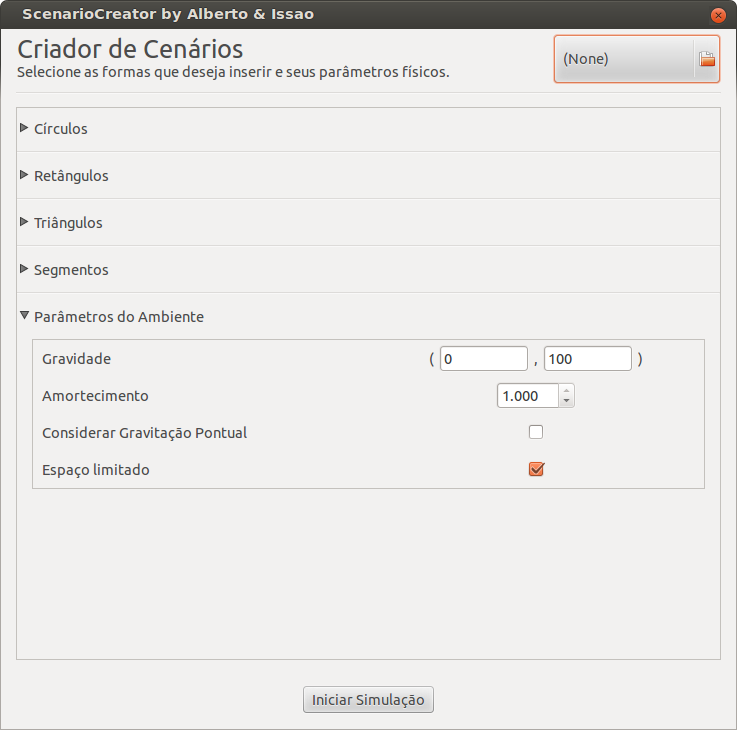
\includegraphics[scale=0.5]{telaInicial.png}
  \caption{Tela inicial do Physimulation}
\end{figure}
